%%%%%%%%%%%%%%%%%%%%%%%%%%%%%%%%%%%%%%%%%
% Short Sectioned Assignment
% LaTeX Template
% Version 1.0 (5/5/12)
%
% This template has been downloaded from:
% http://www.LaTeXTemplates.com
%
% Original author:
% Frits Wenneker (http://www.howtotex.com)
%
% License:
% CC BY-NC-SA 3.0 (http://creativecommons.org/licenses/by-nc-sa/3.0/)
%
%%%%%%%%%%%%%%%%%%%%%%%%%%%%%%%%%%%%%%%%%

%----------------------------------------------------------------------------------------
%	PACKAGES AND OTHER DOCUMENT CONFIGURATIONS
%----------------------------------------------------------------------------------------

\documentclass[paper=a4, fontsize=11pt]{scrartcl} % A4 paper and 11pt font size

\usepackage[T1]{fontenc} % Use 8-bit encoding that has 256 glyphs
\usepackage{fourier} % Use the Adobe Utopia font for the document - comment this line to return to the LaTeX default
\usepackage[english]{babel} % English language/hyphenation
\usepackage{amsmath,amsfonts,amsthm} % Math packages
\usepackage{graphicx}
\usepackage{lipsum} % Used for inserting dummy 'Lorem ipsum' text into the template

\usepackage{sectsty} % Allows customizing section commands
\allsectionsfont{\centering \normalfont\scshape} % Make all sections centered, the default font and small caps

\usepackage{fancyhdr} % Custom headers and footers
\pagestyle{fancyplain} % Makes all pages in the document conform to the custom headers and footers
\fancyhead{} % No page header - if you want one, create it in the same way as the footers below
\fancyfoot[L]{} % Empty left footer
\fancyfoot[C]{} % Empty center footer
\fancyfoot[R]{\thepage} % Page numbering for right footer
\renewcommand{\headrulewidth}{0pt} % Remove header underlines
\renewcommand{\footrulewidth}{0pt} % Remove footer underlines
\setlength{\headheight}{13.6pt} % Customize the height of the header

\numberwithin{equation}{section} % Number equations within sections (i.e. 1.1, 1.2, 2.1, 2.2 instead of 1, 2, 3, 4)
\numberwithin{figure}{section} % Number figures within sections (i.e. 1.1, 1.2, 2.1, 2.2 instead of 1, 2, 3, 4)
\numberwithin{table}{section} % Number tables within sections (i.e. 1.1, 1.2, 2.1, 2.2 instead of 1, 2, 3, 4)

\setlength\parindent{0pt} % Removes all indentation from paragraphs - comment this line for an assignment with lots of text

%----------------------------------------------------------------------------------------
%	TITLE SECTION
%----------------------------------------------------------------------------------------

\newcommand{\horrule}[1]{\rule{\linewidth}{#1}} % Create horizontal rule command with 1 argument of height

\title{	
\normalfont \normalsize 
\textsc{Princeton University} \\ [25pt] % Your university, school and/or department name(s)
\horrule{0.5pt} \\[0.4cm] % Thin top horizontal rule
\huge Summary:\ Algorithms,\ Part\ I \\ % The assignment title
\horrule{2pt} \\[0.5cm] % Thick bottom horizontal rule
}

\author{\textbf{Francisco Manuel Garcia Botella}\\ \textit{fmgarcia@dtic.ua.es}} % Your name

\date{\normalsize\today} % Today's date or a custom date

\begin{document}

\maketitle % Print the title

%----------------------------------------------------------------------------------------
%	PROBLEM 1
%----------------------------------------------------------------------------------------

%------------------------------------------------
\section{Chapter 1: Union-Find}
%------------------------------------------------
\subsection{Before develop Algorithms}
%------------------------------------------------
\begin{enumerate}
\item Model the problem. For example: the main elements of the problem that need to be solved.
\item Find an algorithm to solve it. 
\item Is it fast enough? Or fits in memory? In many cases, the first algorithm is enough, but others not.
\item If not, figure out why. Check the requirements we need to it. (Fast algorithm, or fit memory)
\item Find a new way to address the problem. We find a new algorithm and check if it works fine.
\item Iterate until satisfied. The algorithm works fine.
\end{enumerate}

We will check if the algorithm works fine. Once we have solved and checked the algorithm, we work in optimize this algorithm, and re-check.
%------------------------------------------------
\subsection{Dynamic Connectivity}
%------------------------------------------------
The \textbf{Dynamic Connectivity}(\textbf{DC}) is a data structure that dynamically maintains information about the connected components of a graph.

The set \textit{V} of vertices of the graph is fixed, but the set \textit{E} of edges can change. The three cases, in order of difficulty, are:
\begin{itemize}
\item \textbf{Incremental connectivity}: Edges are only added to the graph
\item \textbf{Decremental connectivity}: Edges are only deleted to the graph.
\item \textbf{Fully connectivity}: Edges can be either added or deleted. 
\end{itemize}

After each addition or deletion of an edge, the DC structure should adapt itself such that it can give quick answers to queries.

%------------------------------------------------
\subsection{Union-Find}
%------------------------------------------------

The \textbf{Union-Find Algorithm}(\textbf{UFA}), is a algorithm which uses a disjoiont-set data structure to solve a problem. For example: We have a set of N elements, we are allowed to merge any two items to consider them equal, i.e., we do that two elements belong to the same group that share the same feature. Too, we are allowed to ask whether two items have the same feature. This algorithm is very slow.

\begin{figure}[!h]
\centering
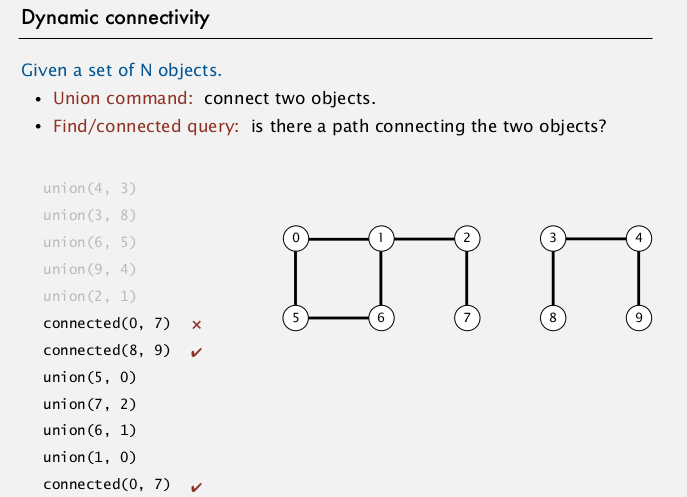
\includegraphics[width=0.8\textwidth]{images/Chapter1/Union-Find.png}
\label{fig:union-find1}
\caption{Example of Union-Find}
\end{figure}


To do this, we use the following functions:
\begin{itemize}
\item \textbf{union(\textit{A},\textit{B})} - Merge A's set with B's set.
\item \textbf{Find(\textit{A})} - Finds what set A belong to.
\item \textbf{Connected(\textit{A},\textit{B})} - Check if A edge is connected with B edge.
\end{itemize}

\subsubsection{Exercise Union-Find}
\textbf{Question 1(Seed = 888220):}
Give the id[] array that results from the following sequence of 6 union
operations on a set of 10 items using the quick-find algorithm.

\begin{center}
4-8 9-0 6-1 8-2 9-3 6-3
\end{center}


Your answer should be a sequence of 10 integers, separated by whitespace.

Recall: our quick-find convention for the union operation p-q is to change id[p]
(and perhaps some other entries) but not id[q].

Response:
The answer is: \textbf{3 3 2 3 2 5 3 7 2 3}

Here is the id[] array after each union operation:
\begin{table}[]
\centering

\label{my-label}
\begin{tabular}{|c|ccllllllll}
\hline
              & \multicolumn{1}{c|}{0} & \multicolumn{1}{c|}{1} & \multicolumn{1}{l|}{\textbf{2}} & \multicolumn{1}{l|}{\textbf{3}} & \multicolumn{1}{l|}{\textbf{4}} & \multicolumn{1}{l|}{\textbf{5}} & \multicolumn{1}{l|}{\textbf{6}} & \multicolumn{1}{l|}{\textbf{7}} & \multicolumn{1}{l|}{\textbf{8}} & \multicolumn{1}{l|}{\textbf{9}} \\ \hline
\textbf{4-8:} & 0                      & 1                      & 2                               & 3                               & 8                               & 5                               & 6                               & 7                               & 8                               & 9                               \\ \cline{1-1}
\textbf{9-0:} & 0                      & 1                      & 2                               & 3                               & 8                               & 5                               & 6                               & 7                               & 8                               & 0                               \\ \cline{1-1}
\textbf{6-1:} & 0                      & 1                      & 2                               & 3                               & 8                               & 5                               & 1                               & 7                               & 8                               & 0                               \\ \cline{1-1}
\textbf{8-2:} & 0                      & 1                      & 2                               & 3                               & 2                               & 5                               & 1                               & 7                               & 2                               & 0                               \\ \cline{1-1}
\textbf{9-3:} & 3                      & 1                      & 2                               & 3                               & 2                               & 5                               & 1                               & 7                               & 2                               & 3                               \\ \cline{1-1}
\textbf{6-3:} & 3                      & 3                      & 2                               & 3                               & 2                               & 5                               & 3                               & 7                               & 2                               & 3                               \\ \cline{1-1}
\end{tabular}
\label{tab:union-find}
\caption{Exercise Union-Find}
\end{table}
%------------------------------------------------
\subsection{Quick Find}
%------------------------------------------------


%------------------------------------------------
\subsection{Quick Union}
%------------------------------------------------
\subsubsection{Exercise Quick-Union}
\textbf{Question 2(seed = 653576):}
Give the id[] array that results from the following sequence of 9 union
operations on a set of 10 items using the weighted quick-union algorithm from lecture.
\begin{center}
9-4 2-5 5-8 1-0 7-2 5-3 4-0 3-0 4-6 
\end{center}
Your answer should be a sequence of 10 integers, separated by whitespace.

Recall: when joining two trees of equal size, our weighted quick union convention is to
make the root of the second tree point to the root of the first tree. Also, our weighted
quick union algorithm performs union by size (number of nodes) -  not union by height -
and does not do path compression.


The correct answer is: 1 9 2 2 9 2 2 2 2 2

Here is the id[] array after each union operation:

\begin{table}[]
\centering
\label{my-label}
\begin{tabular}{c|cccccccccc}
\cline{2-11}
                                    & \multicolumn{1}{c|}{0} & \multicolumn{1}{c|}{1} & \multicolumn{1}{c|}{2} & \multicolumn{1}{c|}{3} & \multicolumn{1}{c|}{4} & \multicolumn{1}{c|}{5} & \multicolumn{1}{c|}{6} & \multicolumn{1}{c|}{7} & \multicolumn{1}{c|}{8} & \multicolumn{1}{c|}{9} \\ \hline
\multicolumn{1}{|c|}{\textbf{9-4:}} & 0                      & 1                      & 2                      & 3                      & 9                      & 5                      & 6                      & 7                      & 8                      & 9                      \\ \cline{1-1}
\multicolumn{1}{|c|}{\textbf{2-5:}} & 0                      & 1                      & 2                      & 3                      & 9                      & 2                      & 6                      & 7                      & 8                      & 9                      \\ \cline{1-1}
\multicolumn{1}{|c|}{\textbf{5-8:}} & 0                      & 1                      & 2                      & 3                      & 9                      & 2                      & 6                      & 7                      & 2                      & 9                      \\ \cline{1-1}
\multicolumn{1}{|c|}{\textbf{1-0:}} & 1                      & 1                      & 2                      & 3                      & 9                      & 2                      & 6                      & 7                      & 2                      & 9                      \\ \cline{1-1}
\multicolumn{1}{|c|}{\textbf{7-2:}} & 1                      & 1                      & 2                      & 3                      & 9                      & 2                      & 6                      & 2                      & 2                      & 9                      \\ \cline{1-1}
\multicolumn{1}{|c|}{\textbf{5-3:}} & 1                      & 1                      & 2                      & 2                      & 9                      & 2                      & 6                      & 2                      & 2                      & 9                      \\ \cline{1-1}
\multicolumn{1}{|c|}{\textbf{4-0:}} & 1                      & 9                      & 2                      & 2                      & 9                      & 2                      & 6                      & 2                      & 2                      & 9                      \\ \cline{1-1}
\multicolumn{1}{|c|}{\textbf{3-0:}} & 1                      & 9                      & 2                      & 2                      & 9                      & 2                      & 6                      & 2                      & 2                      & 2                      \\ \cline{1-1}
\multicolumn{1}{|c|}{\textbf{4-6:}} & 1                      & 9                      & 2                      & 2                      & 9                      & 2                      & 2                      & 2                      & 2                      & 2                      \\ \cline{1-1}
\end{tabular}
\label{tab:exerciseQuickUnion}
\caption{Exercise Quick-Union}
\end{table}


%----------------------------------------------------------------------------------------

\end{document}